\documentclass[aspectratio=169]{beamer}
\usetheme{Madrid}
\usecolortheme{default}

% Packages
\usepackage{graphicx}
\usepackage{amsmath}
\usepackage{amssymb}
\usepackage{tikz}
\usetikzlibrary{arrows,shapes,positioning,calc}
\usepackage{booktabs}
\usepackage{hyperref}
\usepackage{fontawesome5}
\usepackage{xcolor}
\usepackage{listings}

% Code listing settings
\lstset{
  basicstyle=\ttfamily\scriptsize,
  keywordstyle=\color{secondary}\bfseries,
  stringstyle=\color{success},
  commentstyle=\color{gray},
  breaklines=true,
  frame=single,
  backgroundcolor=\color{accent!5},
  rulecolor=\color{secondary!50},
  showstringspaces=false
}

\graphicspath{{./}}

% Custom colors
\definecolor{primary}{RGB}{10,37,64}
\definecolor{secondary}{RGB}{99,91,255}
\definecolor{accent}{RGB}{0,212,255}
\definecolor{success}{RGB}{50,213,131}
\definecolor{warning}{RGB}{255,193,7}
\definecolor{danger}{RGB}{220,53,69}

\setbeamercolor{structure}{fg=secondary}
\setbeamercolor{palette primary}{bg=primary,fg=white}
\setbeamercolor{palette secondary}{bg=secondary,fg=white}
\setbeamercolor{palette tertiary}{bg=accent,fg=white}

% Title page
\title[SE446 - Week 1B]{Project \& Tools Setup}
\subtitle{Big Data Analytics}
\author{Professor Anis Koubaa}
\institute{
    SE 446\\
    Alfaisal University\\[0.3em]
    \url{https://github.com/aniskoubaa/big_data_course}
}
\date{Spring 2026}
\titlegraphic{\includegraphics[width=1.5cm]{logo.png}}

% ============================================
% BEGIN DOCUMENT
% ============================================
\begin{document}

% Title slide
\begin{frame}
\titlepage
\end{frame}

% Outline
\begin{frame}{Today's Agenda}
  \tableofcontents[hideallsubsections]
\end{frame}

% ===========================================
\section{Semester Project Overview}
% ===========================================

\begin{frame}{Smart City Data Platform}
  \begin{block}{Your Mission}
    Build an end-to-end \textbf{Big Data analytics platform} using real urban datasets.
  \end{block}
  
  \vspace{0.5em}
  
  \begin{columns}[T]
    \begin{column}{0.55\textwidth}
      \textbf{What You'll Build:}
      \begin{itemize}
        \item Data ingestion pipelines
        \item MapReduce processing jobs
        \item SQL analytics with Hive
        \item Spark-based transformations
        \item Real-time streaming dashboards
      \end{itemize}
    \end{column}
    
    \begin{column}{0.4\textwidth}
      \centering
      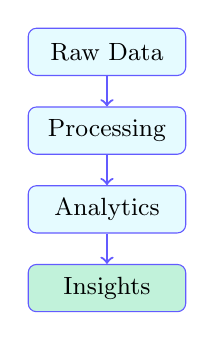
\begin{tikzpicture}[
        box/.style={rectangle, draw=secondary, fill=accent!10, 
                    minimum width=2cm, minimum height=0.6cm, align=center, rounded corners=3pt, font=\small}
      ]
        \node[box] (data) at (0, 2) {Raw Data};
        \node[box] (process) at (0, 1) {Processing};
        \node[box] (analyze) at (0, 0) {Analytics};
        \node[box, fill=success!30] (insight) at (0, -1) {Insights};
        
        \draw[->, thick, secondary] (data) -- (process);
        \draw[->, thick, secondary] (process) -- (analyze);
        \draw[->, thick, secondary] (analyze) -- (insight);
      \end{tikzpicture}
    \end{column}
  \end{columns}
\end{frame}

\begin{frame}{Why a Smart City Project?}
  \centering
  \begin{tikzpicture}[
    box/.style={rectangle, draw=secondary, fill=accent!10, 
                minimum width=2.5cm, minimum height=1cm, align=center, rounded corners=5pt},
    scale=0.9
  ]
    \node[box] (taxi) at (-4, 0) {\faIcon{taxi}\\Transportation};
    \node[box] (crime) at (-1.3, 0) {\faIcon{shield-alt}\\Public Safety};
    \node[box] (weather) at (1.4, 0) {\faIcon{cloud-sun}\\Weather};
    \node[box] (air) at (4.1, 0) {\faIcon{wind}\\Air Quality};
    
    \node[rectangle, draw=success, fill=success!20, 
          minimum width=10cm, minimum height=1.2cm, align=center, rounded corners=5pt] 
          (platform) at (0, -2) {\Large\textbf{Smart City Data Platform}};
    
    \draw[->, thick, secondary] (taxi.south) -- ++(0,-0.5) -| ([xshift=-3cm]platform.north);
    \draw[->, thick, secondary] (crime.south) -- ++(0,-0.5) -| ([xshift=-1cm]platform.north);
    \draw[->, thick, secondary] (weather.south) -- ++(0,-0.5) -| ([xshift=1cm]platform.north);
    \draw[->, thick, secondary] (air.south) -- ++(0,-0.5) -| ([xshift=3cm]platform.north);
  \end{tikzpicture}
  
  \vspace{0.5em}
  
  \begin{block}{Real-World Relevance}
    Smart cities generate \textbf{massive amounts of data}. Learn to process it!
  \end{block}
\end{frame}

% ===========================================
\section{5 Milestones Explained}
% ===========================================

\begin{frame}{Project Milestones Overview}
  \centering
  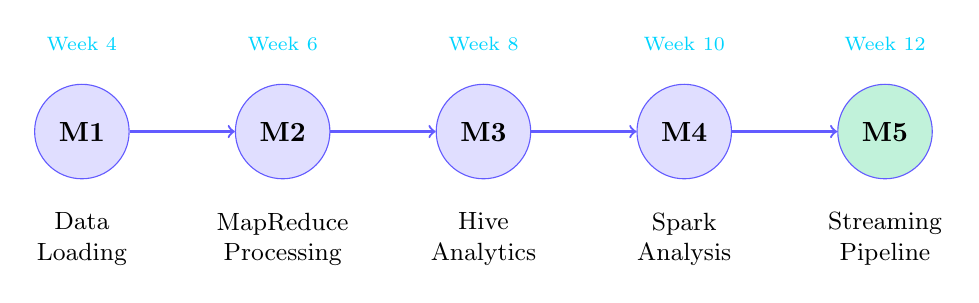
\begin{tikzpicture}[
    ms/.style={circle, draw=secondary, fill=secondary!20, 
               minimum size=1.2cm, font=\bfseries, inner sep=0pt},
    label/.style={align=center, font=\small},
    scale=0.85
  ]
    \node[ms] (m1) at (0, 0) {M1};
    \node[ms] (m2) at (3, 0) {M2};
    \node[ms] (m3) at (6, 0) {M3};
    \node[ms] (m4) at (9, 0) {M4};
    \node[ms, fill=success!30] (m5) at (12, 0) {M5};
    
    \draw[->, thick, secondary] (m1) -- (m2);
    \draw[->, thick, secondary] (m2) -- (m3);
    \draw[->, thick, secondary] (m3) -- (m4);
    \draw[->, thick, secondary] (m4) -- (m5);
    
    \node[label, below=0.3cm of m1] {Data\\Loading};
    \node[label, below=0.3cm of m2] {MapReduce\\Processing};
    \node[label, below=0.3cm of m3] {Hive\\Analytics};
    \node[label, below=0.3cm of m4] {Spark\\Analysis};
    \node[label, below=0.3cm of m5] {Streaming\\Pipeline};
    
    \node[font=\scriptsize, above=0.3cm of m1, accent] {Week 4};
    \node[font=\scriptsize, above=0.3cm of m2, accent] {Week 6};
    \node[font=\scriptsize, above=0.3cm of m3, accent] {Week 8};
    \node[font=\scriptsize, above=0.3cm of m4, accent] {Week 10};
    \node[font=\scriptsize, above=0.3cm of m5, accent] {Week 12};
  \end{tikzpicture}
  
  \vspace{1em}
  
  \begin{tabular}{ccc}
    \toprule
    \textbf{Each Milestone} & \textbf{Weight} & \textbf{Total} \\
    \midrule
    4\% & × 5 milestones & = 20\% of course grade \\
    \bottomrule
  \end{tabular}
\end{frame}

\begin{frame}{M1: Data Loading (Week 4)}
  \begin{columns}[T]
    \begin{column}{0.55\textwidth}
      \begin{block}{Objective}
        Load and explore datasets in a distributed environment
      \end{block}
      
      \vspace{0.3em}
      
      \textbf{Key Tasks:}
      \begin{itemize}
        \item Understand HDFS concepts
        \item Load CSV/JSON files
        \item Explore data schemas
        \item Basic data profiling
        \item Handle missing values
      \end{itemize}
    \end{column}
    
    \begin{column}{0.4\textwidth}
      \begin{block}{Technologies}
        \begin{itemize}
          \item Google Colab
          \item Pandas basics
          \item HDFS concepts
          \item Data formats
        \end{itemize}
      \end{block}
      
      \vspace{0.3em}
      
      \textbf{Deliverable:}\\
      Jupyter notebook with data loaded and explored
    \end{column}
  \end{columns}
\end{frame}

\begin{frame}{M1: Smart City Context}
  \begin{block}{\faIcon{city} Why This Matters for Smart Cities}
    Cities collect \textbf{millions of records daily} from taxis, sensors, and systems. Before any analysis, data must be loaded and understood.
  \end{block}
  
  \vspace{0.5em}
  
  \begin{columns}[T]
    \begin{column}{0.48\textwidth}
      \textbf{Real-World Problem:}
      \begin{itemize}
        \item NYC Taxi: 400K+ trips/day
        \item Data arrives in various formats
        \item Missing values common
        \item Schema changes over time
      \end{itemize}
    \end{column}
    
    \begin{column}{0.48\textwidth}
      \textbf{Why Big Data Tools?}
      \begin{itemize}
        \item Excel can't handle 1M+ rows
        \item Need distributed storage (HDFS)
        \item Automated profiling essential
        \item Scalable from day one
      \end{itemize}
    \end{column}
  \end{columns}
  
  \vspace{0.5em}
  
  \begin{block}{Learning Outcome}
    Understand how to prepare urban data for analysis at scale.
  \end{block}
\end{frame}

\begin{frame}[fragile]{M1: Sample Code Preview}
  \begin{columns}[T]
    \begin{column}{0.58\textwidth}
      \begin{block}{Loading and Exploring Data with Pandas}
      \end{block}
      \begin{lstlisting}[language=Python]
import pandas as pd

# Load the NYC Taxi dataset
df = pd.read_csv('nyc_taxi_data.csv')

# Display basic info
print(f"Shape: {df.shape}")
print(df.columns.tolist())

# Check for missing values
print(df.isnull().sum())

# Basic statistics
print(df.describe())
      \end{lstlisting}
    \end{column}
    
    \begin{column}{0.38\textwidth}
      \begin{block}{What You'll Learn}
        \begin{itemize}
          \item Load CSV/JSON data
          \item Explore data schemas
          \item Handle missing values
          \item Basic data profiling
          \item Pandas DataFrame ops
        \end{itemize}
      \end{block}
      
      \vspace{0.5em}
      
      \begin{block}{Key Concepts}
        \texttt{read\_csv()}, \texttt{shape}, \texttt{isnull()}, \texttt{describe()}
      \end{block}
    \end{column}
  \end{columns}
\end{frame}

\begin{frame}{M2: MapReduce Processing (Week 6)}
  \begin{columns}[T]
    \begin{column}{0.55\textwidth}
      \begin{block}{Objective}
        Implement batch processing with MapReduce paradigm
      \end{block}
      
      \vspace{0.3em}
      
      \textbf{Key Tasks:}
      \begin{itemize}
        \item Write custom mappers
        \item Write custom reducers
        \item Aggregation operations
        \item Word count patterns
        \item Data transformations
      \end{itemize}
    \end{column}
    
    \begin{column}{0.4\textwidth}
      \begin{block}{Technologies}
        \begin{itemize}
          \item MapReduce concepts
          \item mrjob (Python)
          \item Databricks
        \end{itemize}
      \end{block}
      
      \vspace{0.3em}
      
      \textbf{Deliverable:}\\
      MapReduce jobs processing taxi/crime data
    \end{column}
  \end{columns}
\end{frame}

\begin{frame}{M2: Smart City Context}
  \begin{block}{\faIcon{shield-alt} Why This Matters for Smart Cities}
    \textbf{Crime analysis} requires processing millions of incident records to identify patterns, hotspots, and trends.
  \end{block}
  
  \vspace{0.5em}
  
  \begin{columns}[T]
    \begin{column}{0.48\textwidth}
      \textbf{Real-World Problem:}
      \begin{itemize}
        \item Chicago: 500K+ crime records/year
        \item Need to count by type, location
        \item Traditional SQL too slow
        \item Single machine can't scale
      \end{itemize}
    \end{column}
    
    \begin{column}{0.48\textwidth}
      \textbf{Why MapReduce?}
      \begin{itemize}
        \item Parallel processing across nodes
        \item Fault-tolerant execution
        \item Scales horizontally
        \item Perfect for batch aggregation
      \end{itemize}
    \end{column}
  \end{columns}
  
  \vspace{0.5em}
  
  \begin{block}{Learning Outcome}
    Learn to parallelize computations when data is too large for one machine.
  \end{block}
\end{frame}

\begin{frame}[fragile]{M2: Sample Code Preview}
  \begin{columns}[T]
    \begin{column}{0.58\textwidth}
      \begin{block}{MapReduce: Count Crimes by Type}
      \end{block}
      \begin{lstlisting}[language=Python]
from mrjob.job import MRJob

class CrimeTypeCount(MRJob):
    
    def mapper(self, _, line):
        if not line.startswith('ID'):
            fields = line.split(',')
            crime_type = fields[5]
            yield crime_type, 1
    
    def reducer(self, key, counts):
        yield key, sum(counts)

if __name__ == '__main__':
    CrimeTypeCount.run()
      \end{lstlisting}
    \end{column}
    
    \begin{column}{0.38\textwidth}
      \begin{block}{What You'll Learn}
        \begin{itemize}
          \item Map function (key-value)
          \item Reduce function (aggregate)
          \item Distributed processing
          \item Data transformations
        \end{itemize}
      \end{block}
      
      \vspace{0.5em}
      
      \begin{block}{Key Concepts}
        \texttt{mapper()}, \texttt{reducer()}, \texttt{yield}, word count pattern
      \end{block}
    \end{column}
  \end{columns}
\end{frame}

\begin{frame}{M3: Hive Analytics (Week 8)}
  \begin{columns}[T]
    \begin{column}{0.55\textwidth}
      \begin{block}{Objective}
        Perform SQL analytics on Big Data using Hive
      \end{block}
      
      \vspace{0.3em}
      
      \textbf{Key Tasks:}
      \begin{itemize}
        \item Create Hive tables
        \item Write HiveQL queries
        \item Joins and aggregations
        \item Partitioning strategies
        \item Performance optimization
      \end{itemize}
    \end{column}
    
    \begin{column}{0.4\textwidth}
      \begin{block}{Technologies}
        \begin{itemize}
          \item Apache Hive
          \item HiveQL (SQL-like)
          \item Databricks SQL
        \end{itemize}
      \end{block}
      
      \vspace{0.3em}
      
      \textbf{Deliverable:}\\
      Analytics queries answering business questions
    \end{column}
  \end{columns}
\end{frame}

\begin{frame}{M3: Smart City Context}
  \begin{block}{\faIcon{taxi} Why This Matters for Smart Cities}
    City planners need \textbf{SQL-like analytics} on transportation data to optimize routes, pricing, and schedules.
  \end{block}
  
  \vspace{0.5em}
  
  \begin{columns}[T]
    \begin{column}{0.48\textwidth}
      \textbf{Real-World Problem:}
      \begin{itemize}
        \item Find peak hours for taxi demand
        \item Calculate average fares by zone
        \item Identify underserved areas
        \item Optimize fleet allocation
      \end{itemize}
    \end{column}
    
    \begin{column}{0.48\textwidth}
      \textbf{Why Hive/SQL?}
      \begin{itemize}
        \item Familiar SQL syntax
        \item Runs on distributed data
        \item Business users can query
        \item No coding required
      \end{itemize}
    \end{column}
  \end{columns}
  
  \vspace{0.5em}
  
  \begin{block}{Learning Outcome}
    Enable business analysts to query Big Data without programming.
  \end{block}
\end{frame}

\begin{frame}[fragile]{M3: Sample Code Preview}
  \begin{columns}[T]
    \begin{column}{0.58\textwidth}
      \begin{block}{HiveQL: Analyze Taxi Trip Patterns}
      \end{block}
      \begin{lstlisting}[language=SQL]
-- Create external table
CREATE EXTERNAL TABLE taxi_trips (
    pickup_datetime STRING,
    passenger_count INT,
    trip_distance DOUBLE,
    fare_amount DOUBLE
) ROW FORMAT DELIMITED 
  FIELDS TERMINATED BY ',';

-- Average fare by hour
SELECT HOUR(pickup_datetime) as hr,
       AVG(fare_amount) as avg_fare
FROM taxi_trips
GROUP BY HOUR(pickup_datetime);
      \end{lstlisting}
    \end{column}
    
    \begin{column}{0.38\textwidth}
      \begin{block}{What You'll Learn}
        \begin{itemize}
          \item Create Hive tables
          \item SQL on Big Data
          \item Aggregations (AVG, COUNT)
          \item Time-based analysis
        \end{itemize}
      \end{block}
      
      \vspace{0.5em}
      
      \begin{block}{Key Concepts}
        \texttt{CREATE TABLE}, \texttt{GROUP BY}, \texttt{HOUR()}, external tables
      \end{block}
    \end{column}
  \end{columns}
\end{frame}

\begin{frame}{M4: Spark Analysis (Week 10)}
  \begin{columns}[T]
    \begin{column}{0.55\textwidth}
      \begin{block}{Objective}
        Leverage Spark for advanced data processing
      \end{block}
      
      \vspace{0.3em}
      
      \textbf{Key Tasks:}
      \begin{itemize}
        \item PySpark DataFrames
        \item Spark SQL queries
        \item Data transformations
        \item Joining multiple datasets
        \item Performance tuning
      \end{itemize}
    \end{column}
    
    \begin{column}{0.4\textwidth}
      \begin{block}{Technologies}
        \begin{itemize}
          \item Apache Spark
          \item PySpark
          \item Spark SQL
          \item Databricks
        \end{itemize}
      \end{block}
      
      \vspace{0.3em}
      
      \textbf{Deliverable:}\\
      Spark notebook with multi-dataset analysis
    \end{column}
  \end{columns}
\end{frame}

\begin{frame}{M4: Smart City Context}
  \begin{block}{\faIcon{cloud-sun} Why This Matters for Smart Cities}
    Understanding \textbf{cross-domain correlations} (weather $\times$ transportation) improves city services.
  \end{block}
  
  \vspace{0.5em}
  
  \begin{columns}[T]
    \begin{column}{0.48\textwidth}
      \textbf{Real-World Problem:}
      \begin{itemize}
        \item How does rain affect taxi tips?
        \item Do snow days increase demand?
        \item Air quality impact on ridership?
        \item Need to join multiple datasets
      \end{itemize}
    \end{column}
    
    \begin{column}{0.48\textwidth}
      \textbf{Why Apache Spark?}
      \begin{itemize}
        \item 100x faster than MapReduce
        \item In-memory processing
        \item Easy joins across datasets
        \item Python-friendly (PySpark)
      \end{itemize}
    \end{column}
  \end{columns}
  
  \vspace{0.5em}
  
  \begin{block}{Learning Outcome}
    Combine multiple data sources to discover urban insights.
  \end{block}
\end{frame}

\begin{frame}[fragile]{M4: Sample Code Preview}
  \begin{columns}[T]
    \begin{column}{0.58\textwidth}
      \begin{block}{PySpark: Join Taxi with Weather}
      \end{block}
      \begin{lstlisting}[language=Python]
from pyspark.sql import SparkSession
from pyspark.sql.functions import *

spark = SparkSession.builder \
    .appName("TaxiWeather").getOrCreate()

# Load datasets
taxi = spark.read.csv("taxi.csv", header=True)
weather = spark.read.csv("weather.csv", header=True)

# Join on date
joined = taxi.join(weather,
    to_date(taxi.pickup_datetime) == weather.date)

# Analyze by precipitation
joined.groupBy("precipitation") \
    .agg(avg("tip_amount")).show()
      \end{lstlisting}
    \end{column}
    
    \begin{column}{0.38\textwidth}
      \begin{block}{What You'll Learn}
        \begin{itemize}
          \item PySpark DataFrames
          \item Multi-dataset joins
          \item Spark SQL functions
          \item Data transformations
        \end{itemize}
      \end{block}
      
      \vspace{0.5em}
      
      \begin{block}{Key Concepts}
        \texttt{SparkSession}, \texttt{join()}, \texttt{groupBy()}, \texttt{agg()}
      \end{block}
    \end{column}
  \end{columns}
\end{frame}

\begin{frame}{M5: Streaming Pipeline (Week 12)}
  \begin{columns}[T]
    \begin{column}{0.55\textwidth}
      \begin{block}{Objective}
        Build a real-time data streaming pipeline
      \end{block}
      
      \vspace{0.3em}
      
      \textbf{Key Tasks:}
      \begin{itemize}
        \item Kafka producer/consumer
        \item Spark Structured Streaming
        \item Real-time aggregations
        \item Window operations
        \item Dashboard visualization
      \end{itemize}
    \end{column}
    
    \begin{column}{0.4\textwidth}
      \begin{block}{Technologies}
        \begin{itemize}
          \item Apache Kafka
          \item Spark Streaming
          \item Delta Lake
          \item Databricks
        \end{itemize}
      \end{block}
      
      \vspace{0.3em}
      
      \textbf{Deliverable:}\\
      Complete streaming pipeline with visualization
    \end{column}
  \end{columns}
\end{frame}

\begin{frame}{M5: Smart City Context}
  \begin{block}{\faIcon{broadcast-tower} Why This Matters for Smart Cities}
    Real-time monitoring enables \textbf{immediate response} to traffic, emergencies, and service disruptions.
  \end{block}
  
  \vspace{0.5em}
  
  \begin{columns}[T]
    \begin{column}{0.48\textwidth}
      \textbf{Real-World Problem:}
      \begin{itemize}
        \item Live taxi demand tracking
        \item Traffic congestion alerts
        \item Emergency response dispatch
        \item Surge pricing triggers
      \end{itemize}
    \end{column}
    
    \begin{column}{0.48\textwidth}
      \textbf{Why Streaming?}
      \begin{itemize}
        \item Batch processing too slow
        \item Decisions in seconds, not hours
        \item Continuous data ingestion
        \item Real-time dashboards
      \end{itemize}
    \end{column}
  \end{columns}
  
  \vspace{0.5em}
  
  \begin{block}{Learning Outcome}
    Build systems that react to city events as they happen.
  \end{block}
\end{frame}

\begin{frame}[fragile]{M5: Sample Code Preview}
  \begin{columns}[T]
    \begin{column}{0.58\textwidth}
      \begin{block}{Spark Streaming: Real-time Monitoring}
      \end{block}
      \begin{lstlisting}[language=Python]
from pyspark.sql.functions import *

# Read streaming data from Kafka
stream = spark.readStream \
    .format("kafka") \
    .option("subscribe", "taxi_events") \
    .load()

# Count trips per 5-min window
counts = stream \
    .withWatermark("ts", "10 min") \
    .groupBy(window("ts", "5 min")) \
    .count()

# Output to dashboard
counts.writeStream \
    .format("console").start()
      \end{lstlisting}
    \end{column}
    
    \begin{column}{0.38\textwidth}
      \begin{block}{What You'll Learn}
        \begin{itemize}
          \item Kafka integration
          \item Structured Streaming
          \item Window operations
          \item Real-time aggregations
        \end{itemize}
      \end{block}
      
      \vspace{0.5em}
      
      \begin{block}{Key Concepts}
        \texttt{readStream}, \texttt{window()}, \texttt{watermark}, \texttt{writeStream}
      \end{block}
    \end{column}
  \end{columns}
\end{frame}

% ===========================================
\section{Why Big Data Tools?}
% ===========================================

\begin{frame}{Why Can't We Just Use Python/Pandas?}
  \begin{block}{\faIcon{exclamation-triangle} The Problem with Traditional Approaches}
    Our Lab 01 notebook demonstrates fundamental limitations when scaling to real data.
  \end{block}
  
  \vspace{0.3em}
  
  \begin{columns}[T]
    \begin{column}{0.48\textwidth}
      \textbf{1. Algorithmic Complexity}
      \begin{itemize}
        \item O(n²) nested loops
        \item 50 records → 2,500 comparisons
        \item 1M records → \textcolor{red}{\textbf{1 trillion!}}
        \item Estimated time: \textcolor{red}{\textbf{34+ hours}}
      \end{itemize}
      
      \vspace{0.3em}
      
      \textbf{2. Memory Limits}
      \begin{itemize}
        \item 50 records → 17 KB RAM
        \item 100M records → \textcolor{red}{\textbf{33 GB RAM}}
        \item Your laptop: 8-16 GB
      \end{itemize}
    \end{column}
    
    \begin{column}{0.48\textwidth}
      \textbf{3. Single-Threaded Processing}
      \begin{itemize}
        \item Pandas uses 1 CPU core
        \item Modern servers: 64+ cores idle
        \item 100M records: 51 seconds
        \item With Spark: \textcolor{green!60!black}{\textbf{0.5 sec}}
      \end{itemize}
      
      \vspace{0.3em}
      
      \textbf{4. No Fault Tolerance}
      \begin{itemize}
        \item Crash = start over
        \item No automatic recovery
        \item Days of work lost
      \end{itemize}
    \end{column}
  \end{columns}
  
  \vspace{0.3em}
  
  \centering
  \small\textit{Try it yourself in Lab 01 notebook!}
\end{frame}

\begin{frame}{Big Data Tools Solve These Problems \faIcon{check-circle}}
  \centering
  \small
  \begin{tabular}{p{2.8cm}p{2.8cm}p{5.5cm}}
    \toprule
    \textbf{Problem} & \textbf{Traditional} & \textbf{Big Data Solution} \\
    \midrule
    \faIcon{hourglass-half} O(n²) Complexity & \textcolor{red}{Hours/Days} & \textbf{MapReduce:} Parallelize across 100+ nodes \\
    \addlinespace
    \faIcon{memory} Memory Limits & \textcolor{red}{Can't load} & \textbf{HDFS:} Distribute storage across cluster \\
    \addlinespace
    \faIcon{microchip} Single CPU & \textcolor{red}{Wastes 63 cores} & \textbf{Spark:} Use all cores on all machines \\
    \addlinespace
    \faIcon{bolt} No Recovery & \textcolor{red}{Start over} & \textbf{Hadoop:} Auto-recover from failures \\
    \bottomrule
  \end{tabular}
  
  \vspace{0.8em}
  
  \begin{block}{\faIcon{lightbulb} Key Insight}
    The same Pandas-like code runs on \textbf{Spark/Databricks}—the infrastructure handles scaling!
  \end{block}
  
  \vspace{0.3em}
  
  \small\textit{This is why we learn Hadoop, MapReduce, Hive, and Spark in this course.}
\end{frame}

% ===========================================
\section{Datasets Overview}
% ===========================================

\begin{frame}{Datasets We'll Use}
  \centering
  \begin{tabular}{llll}
    \toprule
    \textbf{Dataset} & \textbf{Size} & \textbf{Records} & \textbf{Description} \\
    \midrule
    \textcolor{warning}{NYC Yellow Taxi} & $\sim$50 MB & 1M+ trips & Trip records, fares, locations \\
    \textcolor{danger}{Chicago Crimes} & $\sim$30 MB & 500K+ & Crime types, dates, GPS coords \\
    \textcolor{accent}{NYC Weather} & $\sim$5 MB & 10K+ & Daily temp, precipitation \\
    \textcolor{success}{Air Quality Index} & $\sim$3 MB & 5K+ & Daily AQI by city \\
    \bottomrule
  \end{tabular}
  
  \vspace{1em}
  
  \begin{columns}
    \begin{column}{0.48\textwidth}
      \begin{block}{\faIcon{check-circle} Pre-Hosted}
        All datasets are already hosted. No downloading needed!
      \end{block}
    \end{column}
    
    \begin{column}{0.48\textwidth}
      \begin{block}{\faIcon{database} Real Data}
        Based on actual open government data sources.
      \end{block}
    \end{column}
  \end{columns}
\end{frame}

\begin{frame}{Where Are Datasets Hosted?}
  \begin{block}{\faIcon{kaggle} Original Source: Kaggle}
    Full datasets available on Kaggle (free account required)
  \end{block}
  
  \vspace{0.3em}
  
  {\small
  \begin{tabular}{ll}
    \toprule
    \textbf{Dataset} & \textbf{Kaggle Link} \\
    \midrule
    NYC Yellow Taxi & \url{kaggle.com/datasets/elemento/nyc-yellow-taxi-trip-data} \\
    Chicago Crimes & \url{kaggle.com/datasets/chicago/chicago-crime} \\
    NYC Weather & \url{kaggle.com/datasets/danbraswell/new-york-city-weather-data-2019} \\
    Air Quality Index & \url{kaggle.com/datasets/programmerrdai/air-quality-data-2012-to-2024} \\
    \bottomrule
  \end{tabular}
  }
  
  \vspace{0.5em}
  
  \begin{columns}[T]
    \begin{column}{0.48\textwidth}
      \begin{block}{\faIcon{github} Course Samples}
        \textbf{Small CSV samples} provided in:\\
        \texttt{github.com/aniskoubaa/\\big\_data\_course/data/}
      \end{block}
    \end{column}
    
    \begin{column}{0.48\textwidth}
      \begin{block}{\faIcon{laptop-code} For Class Work}
        \begin{itemize}
          \item Use GitHub samples for testing
          \item Use Kaggle for full analysis
          \item Both work in Colab/Databricks
        \end{itemize}
      \end{block}
    \end{column}
  \end{columns}
\end{frame}

\begin{frame}{NYC Yellow Taxi Dataset}
  \begin{columns}[T]
    \begin{column}{0.5\textwidth}
      \textbf{Key Fields:}
      \begin{itemize}
        \item \texttt{pickup\_datetime} - When trip started
        \item \texttt{dropoff\_datetime} - When trip ended
        \item \texttt{passenger\_count} - Number of passengers
        \item \texttt{trip\_distance} - Miles traveled
        \item \texttt{fare\_amount} - Base fare
        \item \texttt{tip\_amount} - Tip given
        \item \texttt{pickup\_location} - Start zone
        \item \texttt{dropoff\_location} - End zone
      \end{itemize}
    \end{column}
    
    \begin{column}{0.45\textwidth}
      \begin{block}{Sample Questions}
        \begin{itemize}
          \item What's the average trip distance?
          \item Which hours are busiest?
          \item How do tips vary by time of day?
          \item Most popular pickup locations?
        \end{itemize}
      \end{block}
    \end{column}
  \end{columns}
\end{frame}

\begin{frame}{NYC Yellow Taxi - Sample Data}
  \centering
  \textbf{Sample Records from \texttt{nyc\_taxi\_data.csv}}
  
  \vspace{0.5em}
  
  {\scriptsize
  \begin{tabular}{llcccc}
    \toprule
    \textbf{pickup\_datetime} & \textbf{dropoff\_datetime} & \textbf{passengers} & \textbf{distance} & \textbf{fare} & \textbf{tip} \\
    \midrule
    2024-01-15 08:23:00 & 2024-01-15 08:45:00 & 2 & 3.5 & 18.50 & 4.00 \\
    2024-01-15 09:10:00 & 2024-01-15 09:25:00 & 1 & 1.8 & 12.00 & 2.50 \\
    2024-01-15 12:45:00 & 2024-01-15 13:30:00 & 3 & 8.2 & 32.00 & 6.40 \\
    2024-01-15 18:00:00 & 2024-01-15 18:15:00 & 1 & 2.1 & 14.50 & 3.00 \\
    2024-01-15 22:30:00 & 2024-01-15 23:00:00 & 4 & 5.6 & 25.00 & 5.00 \\
    \bottomrule
  \end{tabular}
  }
  
  \vspace{1em}
  
  \begin{block}{Data Insights}
    \begin{itemize}
      \item \textbf{1M+ records} spanning several months
      \item Timestamps allow time-based analysis (rush hours, weekends)
      \item Fare and tip data enable financial analysis
    \end{itemize}
  \end{block}
\end{frame}

\begin{frame}{Chicago Crimes Dataset}
  \begin{columns}[T]
    \begin{column}{0.5\textwidth}
      \textbf{Key Fields:}
      \begin{itemize}
        \item \texttt{date} - When crime occurred
        \item \texttt{primary\_type} - Crime category
        \item \texttt{description} - Detailed type
        \item \texttt{location\_description} - Where
        \item \texttt{arrest} - Was arrest made?
        \item \texttt{latitude}, \texttt{longitude} - GPS
        \item \texttt{district} - Police district
      \end{itemize}
    \end{column}
    
    \begin{column}{0.45\textwidth}
      \begin{block}{Sample Questions}
        \begin{itemize}
          \item Most common crime types?
          \item Crime trends by month?
          \item Arrest rate by crime type?
          \item Hotspot locations?
        \end{itemize}
      \end{block}
    \end{column}
  \end{columns}
\end{frame}

\begin{frame}{Chicago Crimes - Sample Data}
  \centering
  \textbf{Sample Records from \texttt{chicago\_crimes.csv}}
  
  \vspace{0.5em}
  
  {\scriptsize
  \begin{tabular}{llllc}
    \toprule
    \textbf{date} & \textbf{primary\_type} & \textbf{location} & \textbf{district} & \textbf{arrest} \\
    \midrule
    2024-01-10 14:30 & THEFT & STREET & 11 & False \\
    2024-01-10 22:15 & BATTERY & APARTMENT & 7 & True \\
    2024-01-11 03:45 & BURGLARY & RESIDENCE & 3 & False \\
    2024-01-11 16:20 & ASSAULT & SIDEWALK & 11 & True \\
    2024-01-12 11:00 & THEFT & RETAIL STORE & 1 & True \\
    \bottomrule
  \end{tabular}
  }
  
  \vspace{1em}
  
  \begin{block}{Data Insights}
    \begin{itemize}
      \item \textbf{500K+ records} with GPS coordinates
      \item 30+ crime types for categorical analysis
      \item Arrest boolean enables outcome analysis
    \end{itemize}
  \end{block}
\end{frame}

\begin{frame}{NYC Weather Dataset}
  \begin{columns}[T]
    \begin{column}{0.5\textwidth}
      \textbf{Key Fields:}
      \begin{itemize}
        \item \texttt{date} - Calendar date
        \item \texttt{temp\_max} - Maximum temperature (°F)
        \item \texttt{temp\_min} - Minimum temperature (°F)
        \item \texttt{temp\_avg} - Average temperature
        \item \texttt{precipitation} - Rainfall (inches)
        \item \texttt{snow} - Snowfall (inches)
        \item \texttt{wind\_speed} - Avg wind speed
      \end{itemize}
    \end{column}
    
    \begin{column}{0.45\textwidth}
      \begin{block}{Sample Questions}
        \begin{itemize}
          \item How does weather affect taxi usage?
          \item Correlation between rain and trips?
          \item Seasonal patterns in ridership?
          \item Snow days vs. normal days?
        \end{itemize}
      \end{block}
    \end{column}
  \end{columns}
\end{frame}

\begin{frame}{NYC Weather - Sample Data}
  \centering
  \textbf{Sample Records from \texttt{nyc\_weather.csv}}
  
  \vspace{0.5em}
  
  {\scriptsize
  \begin{tabular}{lcccccc}
    \toprule
    \textbf{date} & \textbf{temp\_max} & \textbf{temp\_min} & \textbf{temp\_avg} & \textbf{precip} & \textbf{snow} & \textbf{wind} \\
    \midrule
    2024-01-15 & 42 & 28 & 35 & 0.00 & 0.0 & 8.5 \\
    2024-01-16 & 38 & 25 & 31 & 0.25 & 2.1 & 12.3 \\
    2024-01-17 & 35 & 22 & 28 & 0.00 & 0.0 & 6.2 \\
    2024-01-18 & 45 & 32 & 38 & 0.10 & 0.0 & 9.1 \\
    2024-01-19 & 52 & 40 & 46 & 0.50 & 0.0 & 15.4 \\
    \bottomrule
  \end{tabular}
  }
  
  \vspace{1em}
  
  \begin{block}{Data Insights}
    \begin{itemize}
      \item \textbf{10K+ records} spanning multiple years
      \item Perfect for joining with taxi/crime data by date
      \item Enables weather-impact analysis on urban activities
    \end{itemize}
  \end{block}
\end{frame}

\begin{frame}{Air Quality Index Dataset}
  \begin{columns}[T]
    \begin{column}{0.5\textwidth}
      \textbf{Key Fields:}
      \begin{itemize}
        \item \texttt{date} - Measurement date
        \item \texttt{city} - City name
        \item \texttt{aqi\_value} - Air Quality Index (0-500)
        \item \texttt{aqi\_category} - Good/Moderate/Unhealthy
        \item \texttt{main\_pollutant} - PM2.5, Ozone, etc.
        \item \texttt{pm25} - Fine particulate matter
        \item \texttt{ozone} - Ozone level
      \end{itemize}
    \end{column}
    
    \begin{column}{0.45\textwidth}
      \begin{block}{Sample Questions}
        \begin{itemize}
          \item Which cities have worst air quality?
          \item Seasonal AQI patterns?
          \item Correlation with weather?
          \item Days exceeding safety thresholds?
        \end{itemize}
      \end{block}
    \end{column}
  \end{columns}
\end{frame}

\begin{frame}{Air Quality Index - Sample Data}
  \centering
  \textbf{Sample Records from \texttt{air\_quality.csv}}
  
  \vspace{0.5em}
  
  {\scriptsize
  \begin{tabular}{llccll}
    \toprule
    \textbf{date} & \textbf{city} & \textbf{aqi\_value} & \textbf{category} & \textbf{pollutant} & \textbf{pm25} \\
    \midrule
    2024-01-15 & New York & 45 & Good & PM2.5 & 12.3 \\
    2024-01-15 & Chicago & 68 & Moderate & Ozone & 18.5 \\
    2024-01-16 & New York & 82 & Moderate & PM2.5 & 28.1 \\
    2024-01-16 & Chicago & 55 & Moderate & PM2.5 & 15.2 \\
    2024-01-17 & New York & 38 & Good & Ozone & 8.7 \\
    \bottomrule
  \end{tabular}
  }
  
  \vspace{1em}
  
  \begin{block}{Data Insights}
    \begin{itemize}
      \item \textbf{5K+ records} for multiple cities
      \item AQI categories enable health-impact analysis
      \item Can be joined with weather data for correlation studies
    \end{itemize}
  \end{block}
\end{frame}

% ===========================================
\section{GitHub Setup \& Workflow}
% ===========================================

\begin{frame}{Why GitHub?}
  \begin{columns}[T]
    \begin{column}{0.5\textwidth}
      \begin{block}{For You}
        \begin{itemize}
          \item Version control for your code
          \item Backup in the cloud
          \item Portfolio for future jobs
          \item Industry-standard skill
        \end{itemize}
      \end{block}
    \end{column}
    
    \begin{column}{0.45\textwidth}
      \begin{block}{For the Course}
        \begin{itemize}
          \item Track individual contributions
          \item Team collaboration
          \item Code review capability
          \item Submission timestamps
        \end{itemize}
      \end{block}
    \end{column}
  \end{columns}
  
  \vspace{1em}
  
  \centering
  \begin{tikzpicture}
    \node[rectangle, draw=warning, fill=warning!20, rounded corners=5pt, inner sep=10pt] {
      \textbf{\faIcon{exclamation-triangle} Important:} Your GitHub commits are part of your grade!
    };
  \end{tikzpicture}
\end{frame}

\begin{frame}{GitHub Account Setup}
  \begin{enumerate}
    \item Go to \url{https://github.com}
    
    \vspace{0.3em}
    
    \item Click ``Sign Up'' and create account
    
    \vspace{0.3em}
    
    \item \textbf{Username Tips:}
    \begin{itemize}
      \item Use a professional username
      \item Example: \texttt{ahmed-alsaud} or \texttt{fatima\_alfarsi}
      \item \textcolor{danger}{Avoid:} \texttt{coolhacker123}, \texttt{xXx\_gamer}
    \end{itemize}
    
    \vspace{0.3em}
    
    \item Verify your email address
    
    \vspace{0.3em}
    
    \item Apply for \textbf{GitHub Student Developer Pack}:
    \begin{itemize}
      \item \url{https://education.github.com/pack}
      \item Free Pro features with your \texttt{@alfaisal.edu} email
    \end{itemize}
  \end{enumerate}
\end{frame}

\begin{frame}{Team Repository Structure}
  \begin{columns}[T]
    \begin{column}{0.5\textwidth}
      \textbf{Repository Organization:}
      
      \vspace{0.5em}
      
      Each team gets \textbf{ONE shared repository}
      
      \vspace{0.5em}
      
      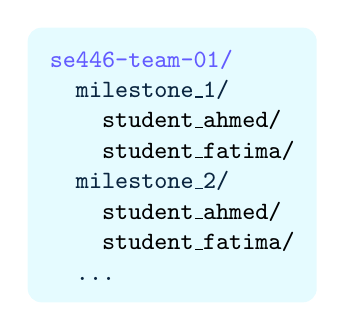
\begin{tikzpicture}[font=\ttfamily\small]
        \node[align=left, fill=accent!10, rounded corners=5pt, inner sep=8pt] at (0,0) {
          \textcolor{secondary}{\textbf{se446-team-01/}}\\
          ~~\textcolor{primary}{milestone\_1/}\\
          ~~~~student\_ahmed/\\
          ~~~~student\_fatima/\\
          ~~\textcolor{primary}{milestone\_2/}\\
          ~~~~student\_ahmed/\\
          ~~~~student\_fatima/\\
          ~~\textcolor{primary}{...}
        };
      \end{tikzpicture}
    \end{column}
    
    \begin{column}{0.45\textwidth}
      \textbf{Important Rules:}
      \begin{itemize}
        \item Each student works in their \textbf{own folder}
        \item Individual commits are tracked separately
        \item Work on your assigned tasks only
        \item Quality matters more than quantity
      \end{itemize}
      
      \vspace{0.5em}
      
      \begin{block}{Note}
        \small Your individual contributions will be evaluated based on your folder's commits
      \end{block}
    \end{column}
  \end{columns}
\end{frame}

\begin{frame}{Essential Git Commands}
  \centering
  \begin{tabular}{ll}
    \toprule
    \textbf{Command} & \textbf{Purpose} \\
    \midrule
    \texttt{git clone <url>} & Download repository \\
    \texttt{git pull} & Get latest changes \\
    \texttt{git status} & Check what's changed \\
    \texttt{git add .} & Stage all changes \\
    \texttt{git commit -m "message"} & Save changes locally \\
    \texttt{git push} & Upload to GitHub \\
    \bottomrule
  \end{tabular}
  
  \vspace{1em}
  
  \begin{block}{Daily Workflow}
    \texttt{git pull} $\rightarrow$ Do work $\rightarrow$ \texttt{git add .} $\rightarrow$ \texttt{git commit -m "M1: ..."} $\rightarrow$ \texttt{git push}
  \end{block}
\end{frame}

\begin{frame}{Commit Message Standards}
  \begin{block}{Format}
    \texttt{<MILESTONE>: <Short description of what you did>}
  \end{block}
  
  \vspace{0.5em}
  
  \begin{columns}[T]
    \begin{column}{0.48\textwidth}
      \textbf{\textcolor{success}{\faIcon{check} Good Examples:}}
      \begin{itemize}
        \item \texttt{M1: Load taxi data and check schema}
        \item \texttt{M2: Implement crime count mapper}
        \item \texttt{M3: Add average fare HiveQL query}
        \item \texttt{M4: Join weather with taxi data}
      \end{itemize}
    \end{column}
    
    \begin{column}{0.48\textwidth}
      \textbf{\textcolor{danger}{\faIcon{times} Bad Examples:}}
      \begin{itemize}
        \item \texttt{update} $\leftarrow$ Too vague
        \item \texttt{asdfasdf} $\leftarrow$ Meaningless
        \item \texttt{done} $\leftarrow$ What's done?
        \item \texttt{fixed stuff} $\leftarrow$ What stuff?
      \end{itemize}
    \end{column}
  \end{columns}
\end{frame}

% ===========================================
\section{Google Colab \& Databricks}
% ===========================================

\begin{frame}{Google Colab Setup}
  \begin{columns}[T]
    \begin{column}{0.5\textwidth}
      \begin{block}{What is Google Colab?}
        Free cloud-based Jupyter notebooks with Python pre-installed.
      \end{block}
      
      \vspace{0.3em}
      
      \textbf{Features:}
      \begin{itemize}
        \item \faIcon{check} No installation needed
        \item \faIcon{check} Python + libraries ready
        \item \faIcon{check} Free GPU access
        \item \faIcon{check} Google Drive integration
        \item \faIcon{check} Easy sharing
      \end{itemize}
    \end{column}
    
    \begin{column}{0.45\textwidth}
      \textbf{Setup Steps:}
      \begin{enumerate}
        \item Go to \url{https://colab.google.com}
        \item Sign in with Google account
        \item Click ``New Notebook''
        \item You're ready!
      \end{enumerate}
      
      \vspace{0.5em}
      
      \begin{block}{We'll Use Colab For:}
        \begin{itemize}
          \item Weeks 1-4
          \item Python \& Pandas basics
          \item M1: Data Loading
        \end{itemize}
      \end{block}
    \end{column}
  \end{columns}
\end{frame}

\begin{frame}{Databricks Community Edition}
  \begin{columns}[T]
    \begin{column}{0.5\textwidth}
      \begin{block}{What is Databricks?}
        Industry-standard cloud platform for Big Data processing with Apache Spark.
      \end{block}
      
      \vspace{0.3em}
      
      \textbf{Features:}
      \begin{itemize}
        \item \faIcon{check} Apache Spark pre-configured
        \item \faIcon{check} Notebooks with clusters
        \item \faIcon{check} Hive, SQL, Streaming
        \item \faIcon{check} Free Community Edition
        \item \faIcon{check} Industry-used platform
      \end{itemize}
    \end{column}
    
    \begin{column}{0.45\textwidth}
      \textbf{Setup Steps:}
      \begin{enumerate}
        \item Go to \url{https://databricks.com/try}
        \item Select ``Community Edition''
        \item Create account (use \texttt{@alfaisal.edu})
        \item Verify email
        \item Create a cluster
      \end{enumerate}
      
      \vspace{0.3em}
      
      \begin{block}{We'll Use Databricks For:}
        \begin{itemize}
          \item Weeks 5-12
          \item M2-M5: MapReduce, Hive, Spark, Streaming
        \end{itemize}
      \end{block}
    \end{column}
  \end{columns}
\end{frame}

\begin{frame}{Colab vs Databricks}
  \centering
  \begin{tabular}{lcc}
    \toprule
    \textbf{Feature} & \textbf{Google Colab} & \textbf{Databricks} \\
    \midrule
    Primary Use & Python/Pandas & Big Data (Spark) \\
    Spark Support & Limited & Native \\
    Setup Difficulty & Easy & Moderate \\
    Cost & Free & Free (Community) \\
    Industry Use & Learning & Production \\
    When We Use & Weeks 1-4 & Weeks 5-12 \\
    \bottomrule
  \end{tabular}
  
  \vspace{1em}
  
  \begin{block}{Bottom Line}
    Start with \textbf{Colab} for basics, graduate to \textbf{Databricks} for real Big Data.
  \end{block}
\end{frame}

% ===========================================
\section{ExamGPT for Submissions}
% ===========================================

\begin{frame}{What is ExamGPT?}
  \begin{columns}[T]
    \begin{column}{0.55\textwidth}
      \begin{block}{Definition}
        ExamGPT is an AI-powered platform for in-class quizzes and submissions.
      \end{block}
      
      \vspace{0.3em}
      
      \textbf{How We'll Use It:}
      \begin{itemize}
        \item Last 15 minutes of each class
        \item Quick comprehension checks
        \item Attendance verification
        \item Instant feedback on answers
      \end{itemize}
      
      \vspace{0.3em}
      
      \textbf{URL:} \url{https://examgpt.aniskoubaa.org}
    \end{column}
    
    \begin{column}{0.4\textwidth}
      \begin{block}{Benefits}
        \begin{itemize}
          \item \faIcon{check} Instant grading
          \item \faIcon{check} AI-powered feedback
          \item \faIcon{check} Tracks your progress
          \item \faIcon{check} Accessible anywhere
        \end{itemize}
      \end{block}
      
      \vspace{0.5em}
      
      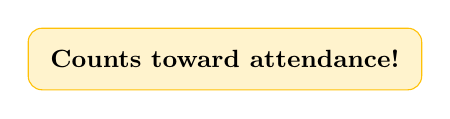
\begin{tikzpicture}
        \node[rectangle, draw=warning, fill=warning!20, rounded corners=5pt, inner sep=8pt] {
          \small\textbf{Counts toward attendance!}
        };
      \end{tikzpicture}
    \end{column}
  \end{columns}
\end{frame}

\begin{frame}{ExamGPT Setup}
  \begin{enumerate}
    \item Go to \url{https://examgpt.aniskoubaa.org}
    
    \vspace{0.3em}
    
    \item Click ``Register'' or ``Sign Up''
    
    \vspace{0.3em}
    
    \item Use your \texttt{@alfaisal.edu} email
    
    \vspace{0.3em}
    
    \item Enter your:
    \begin{itemize}
      \item Full name (as in university records)
      \item Student ID
    \end{itemize}
    
    \vspace{0.3em}
    
    \item Verify your email
    
    \vspace{0.3em}
    
    \item Join the \textbf{SE446} course when prompted
  \end{enumerate}
  
  \vspace{0.5em}
  
  \begin{block}{Important}
    Use the \textbf{same name} as your official university registration!
  \end{block}
\end{frame}

% ===========================================
\section{Setup Checklist \& Q\&A}
% ===========================================

\begin{frame}{Today's Setup Checklist}
  \centering
  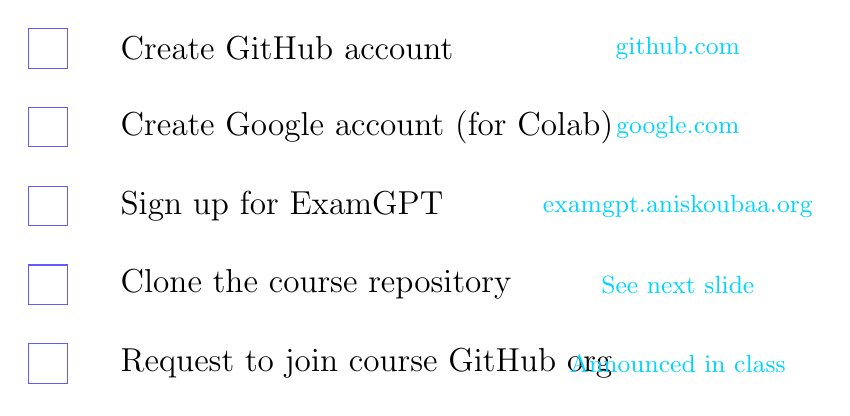
\begin{tikzpicture}[
    checkbox/.style={rectangle, draw=secondary, minimum width=0.5cm, minimum height=0.5cm, inner sep=0pt},
    task/.style={anchor=west, font=\large}
  ]
    \node[checkbox] (c1) at (0, 3) {};
    \node[task] at (0.8, 3) {Create GitHub account};
    \node[font=\small, accent] at (8, 3) {\url{github.com}};
    
    \node[checkbox] (c2) at (0, 2) {};
    \node[task] at (0.8, 2) {Create Google account (for Colab)};
    \node[font=\small, accent] at (8, 2) {\url{google.com}};
    
    \node[checkbox] (c3) at (0, 1) {};
    \node[task] at (0.8, 1) {Sign up for ExamGPT};
    \node[font=\small, accent] at (8, 1) {\url{examgpt.aniskoubaa.org}};
    
    \node[checkbox] (c4) at (0, 0) {};
    \node[task] at (0.8, 0) {Clone the course repository};
    \node[font=\small, accent] at (8, 0) {See next slide};
    
    \node[checkbox] (c5) at (0, -1) {};
    \node[task] at (0.8, -1) {Request to join course GitHub org};
    \node[font=\small, accent] at (8, -1) {Announced in class};
  \end{tikzpicture}
\end{frame}

\begin{frame}{Clone the Course Repository}
  \begin{block}{Course Repository}
    \centering
    \Large\url{https://github.com/aniskoubaa/big_data_course}
  \end{block}
  
  \vspace{0.5em}
  
  \textbf{Option 1: Command Line}
  \begin{itemize}
    \item Open Terminal (Mac/Linux) or Git Bash (Windows)
    \item Run: \texttt{git clone https://github.com/aniskoubaa/big\_data\_course.git}
  \end{itemize}
  
  \vspace{0.3em}
  
  \textbf{Option 2: GitHub Desktop}
  \begin{itemize}
    \item Download from \url{https://desktop.github.com}
    \item Click ``Clone Repository''
    \item Paste the URL
  \end{itemize}
  
  \vspace{0.3em}
  
  \textbf{Option 3: Web Download}
  \begin{itemize}
    \item Click green ``Code'' button on GitHub
    \item Select ``Download ZIP''
  \end{itemize}
\end{frame}

\begin{frame}{Getting Help}
  \begin{columns}[T]
    \begin{column}{0.48\textwidth}
      \begin{block}{During Class}
        \begin{itemize}
          \item Raise your hand
          \item Ask the TA
          \item Help your neighbor
        \end{itemize}
      \end{block}
      
      \vspace{0.3em}
      
      \begin{block}{Office Hours}
        \begin{itemize}
          \item Prof. Koubaa: Office SG-10
          \item By appointment
          \item \texttt{akoubaa@alfaisal.edu}
        \end{itemize}
      \end{block}
    \end{column}
    
    \begin{column}{0.48\textwidth}
      \begin{block}{Online Resources}
        \begin{itemize}
          \item Course GitHub Issues
          \item Moodle Discussion Forum
          \item Google \& Stack Overflow
          \item AI Assistants (for learning)
        \end{itemize}
      \end{block}
      
      \vspace{0.3em}
      
      \begin{block}{Important Links}
        \begin{itemize}
          \item Course: \url{aniskoubaa.org/se446}
          \item Moodle: Alfaisal LMS
        \end{itemize}
      \end{block}
    \end{column}
  \end{columns}
\end{frame}

\begin{frame}{}
  \centering
  \vspace{2em}
  
  {\Huge\textcolor{secondary}{\textbf{Questions?}}}
  
  \vspace{1.5em}
  
  {\Large Let's do the setup together!}
  
  \vspace{1em}
  
  Prof. Anis Koubaa\\
  \texttt{akoubaa@alfaisal.edu}\\[0.5em]
  \url{https://github.com/aniskoubaa/big_data_course}
  
  \vspace{1em}
  
  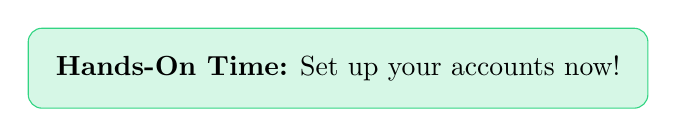
\begin{tikzpicture}
    \node[rectangle, draw=success, fill=success!20, rounded corners=5pt, inner sep=10pt] {
      \textbf{Hands-On Time:} Set up your accounts now!
    };
  \end{tikzpicture}
\end{frame}

\end{document}
